\section{Introduction}
\label{sec:introduction}

Type errors are a common stumbling block for students
trying to learn typed functional languages like \ocaml\
and \haskell.
%
Consider the ill-typed @fac@ function on the left in
Figure~\ref{fig:factorial}.
%
The function returns @true@ in the base case (instead of @1@),
and so \ocaml responds with the error message:
%
% WRW: This used to say 8-23 because you had it spelled "factorial", but
% when it changed to fac, we forgot to update this.
\begin{verbatim}
 File "fac.ml", line 5, characters 8-17:
 Error: This expression has type bool
        but an expression was expected
        of type int
\end{verbatim}
%
This message makes perfect sense to an expert who is familiar
with the language and has a good mental model of how the type
system works.
%
However, it may perplex a novice who has yet to develop such a
mental model.
%
To make matters worse, unification-based type inference algorithms
often report errors far removed from their source.
%
This further increases the novice's confusion and can actively mislead
them to focus their investigation on an irrelevant piece of code.
%
Much recent work has focused on analyzing unification constraints
to properly \emph{localize} a type error~\cite{lerner_searching_2007,chen_counter-factual_2014,zhang_toward_2014,pavlinovic_finding_2014},
but an accurate source location still does not explain \emph{why} the
program is wrong.


\begin{figure}[t]
\centering
\begin{minipage}{.49\linewidth}
\centering
\begin{code}
  let rec fac n =
    if n <= 0 then
      true
    else
      n * fac (n-1)
\end{code}
\end{minipage}
% \hspace{0.3in}
\begin{minipage}{.49\linewidth}
\centering
  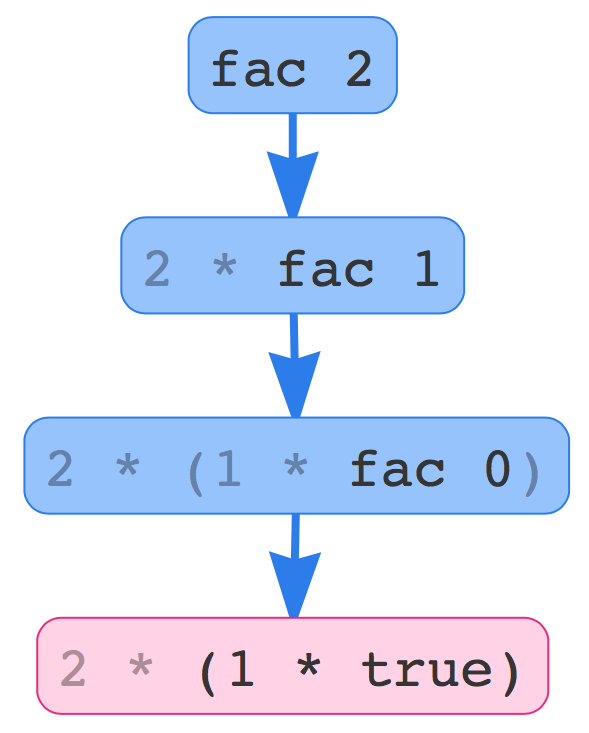
\includegraphics[height=1.5in]{fac-overview.png}
\end{minipage}
\caption{(L) An ill-typed \texttt{fac} function; (R) Dynamically witnessing the type error in \texttt{fac}.}
\label{fig:factorial}
\end{figure}

In this paper we propose a new approach that explains
static type errors by \emph{dynamically} witnessing
how exactly an ill-typed program goes wrong.
%
We have developed \toolname, an interactive tool that uses
the source of the ill-typed function to automatically synthesize
the result on the right in Figure~\ref{fig:factorial}, which
shows how the recursive calls reduce to a configuration where
the program ``goes wrong'' --- \ie\ the @int@ value @1@ is to be
multiplied with the @bool@ value @true@.
We achieve this via three concrete contributions.

\paragraph{1. Finding Witnesses}
Our first contribution is an algorithm for searching for
\emph{witnesses} to type errors, \ie\ inputs that cause a
program to go wrong~(\S~\ref{sec:semantics}).
%
This problem is surprisingly tricky when we cannot rely on
static type information.
%
In particular, we must avoid the trap of \emph{spurious} inputs
that cause irrelevant problems that would be avoided by picking
values of a different, relevant type.
%
We solve this problem by developing a novel operational semantics
that corresponds to executing the program with \emph{holes} ---
values whose type is unknown.
%
Our semantics \emph{conservatively} instantiates holes with concrete
values; thereby dynamically inferring the type of the input
until the program goes wrong.
%
We prove that our procedure synthesizes \emph{general witnesses},
which means, intuitively, that if a witness is found for a given
ill-typed function, then, \emph{for all} input types, there exist
inhabitants that can make the function go wrong.

Given a witness to a type error, the novice may still be at a loss.
%
The standard \ocaml\ interpreter and debugging infrastructure expect
well-typed programs, so they cannot be used to investigate \emph{how}
the witness causes the program to crash.
%
More importantly, the execution itself may be quite long and may contain
details not relevant to the actual error.

\paragraph{2. Visualizing Witnesses}
Our second contribution is a novel interactive visualization of the
execution of \ocaml\ programs, well-typed or not~(\S~\ref{sec:interactive}).
%
We extend the semantics to also build a \emph{reduction graph}
which records all of the small-step reductions and the context
in which they occur.
%
The graph lets us build a visualization that shows a sequence of
steps from the source witness to the stuck term and allows the user
to interactively expand the computation to expose intermediate steps,
by selecting an expression and choosing a traversal strategy.
%
The strategies include many of the standard debugging moves, \eg\
stepping \emph{forward} or \emph{into} or \emph{over} calls, as well
stepping or jumping \emph{backward} to understand how a particular
value was created, while preserving a context of the intermediate
steps that allow the user to keep track of a term's provenance.

\paragraph{3. Evaluating Witnesses}
%
Of course, the problem of finding witnesses is
undecidable. In fact, due to the necessarily
conservative nature of static typing, there
may not even exist any witnesses for a given
ill-typed program.
%
Thus, our approach is a heuristic that is only useful
if it can find \emph{compact} witnesses for
\emph{real-world} programs.
%
Our third contribution is an extensive evaluation of our approach
on two different sets of ill-typed programs obtained by instrumenting
compilers used in beginner's classes~(\S~\ref{sec:evaluation}).
%
The first is the \uwbench\ data set~\cite{lerner_searching_2007}
comprising \uwsize\ ill-typed programs.
%
The second is a new \ucsdbench\ data set, comprising \ucsdsize\
ill-typed programs.
%
We show that for both data sets, our technique is able to generate
witnesses for nearly 90\% of the programs, in under a second the
vast majority of cases.
%
Furthermore, we show that a simple interactive strategy yields
compact counterexample traces with fewer than 5 steps for 60\%
of the programs, and under 10 steps for 90\% of the programs.

\smallskip
Our results show that in the vast majority of
cases, (novices') ill-typed programs \emph{do} go wrong.
This, in turn, opens the door to a novel dynamic way to
explain, understand, and appreciate the benefits of static typing.

%%% Local Variables:
%%% mode: latex
%%% TeX-master: "main"
%%% End:
